\chapter{Implementation}

\section{Modules}
\paragraph{}Implementation of the project is divided into 6 modules as shown in Fig. \ref{modules}.

\begin{figure}[H]
\centering
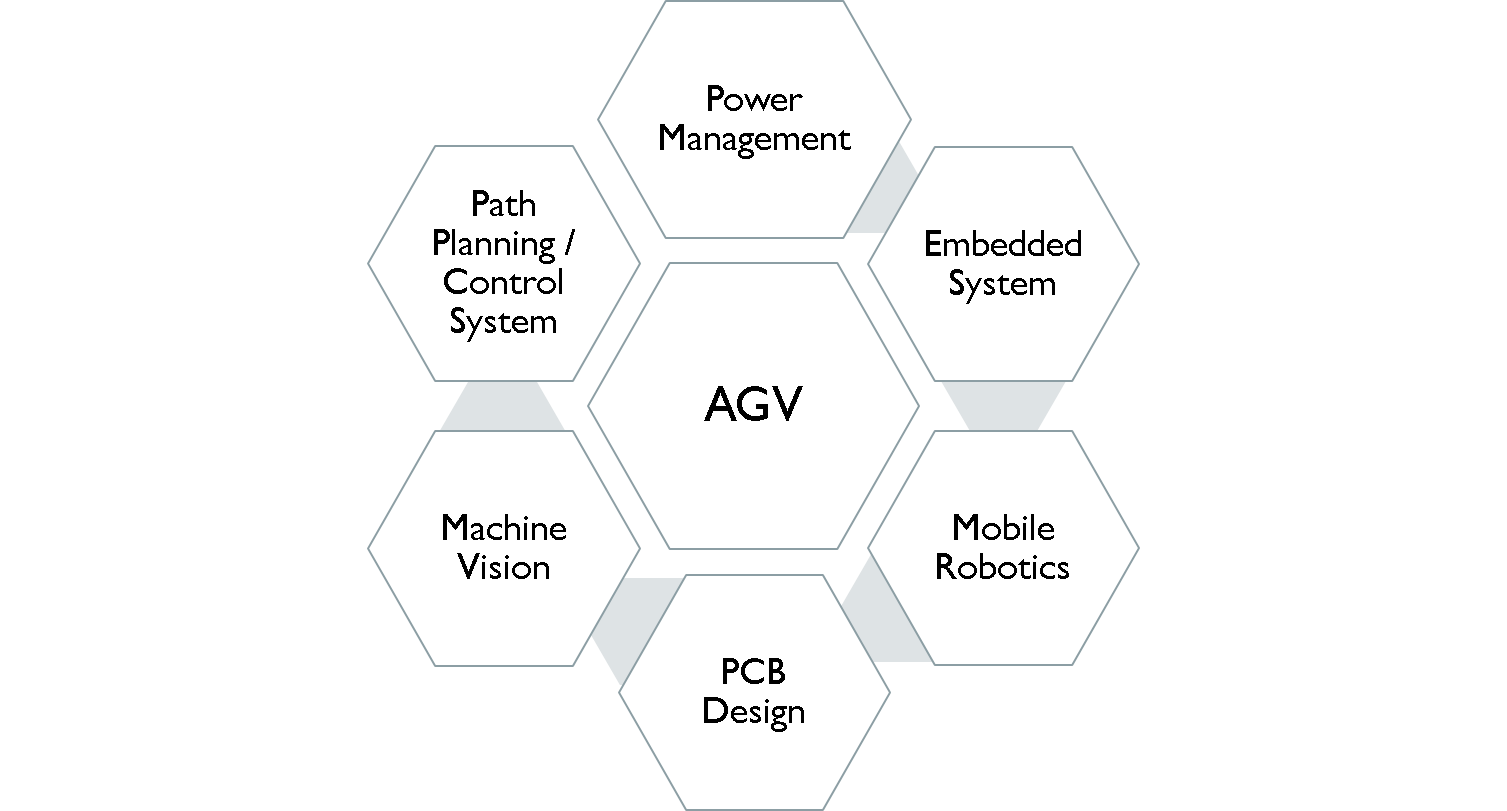
\includegraphics[width = \textwidth]{project/images/modules.png}
\caption{Modules} \label{modules}
\end{figure}

\newpage

\subsection{PCB Design}

\begin{itemize}[wide, labelwidth=!, labelindent=0pt]
    \item \textbf{PCB Schematic}
    \vspace{-0.5cm}
    \paragraph{} We have used Autodesk Eagle for designing project PCB. Schmatic consists of multiple circuit diagram that has to be used in PCB.

    \begin{figure}[H]
    \centering
    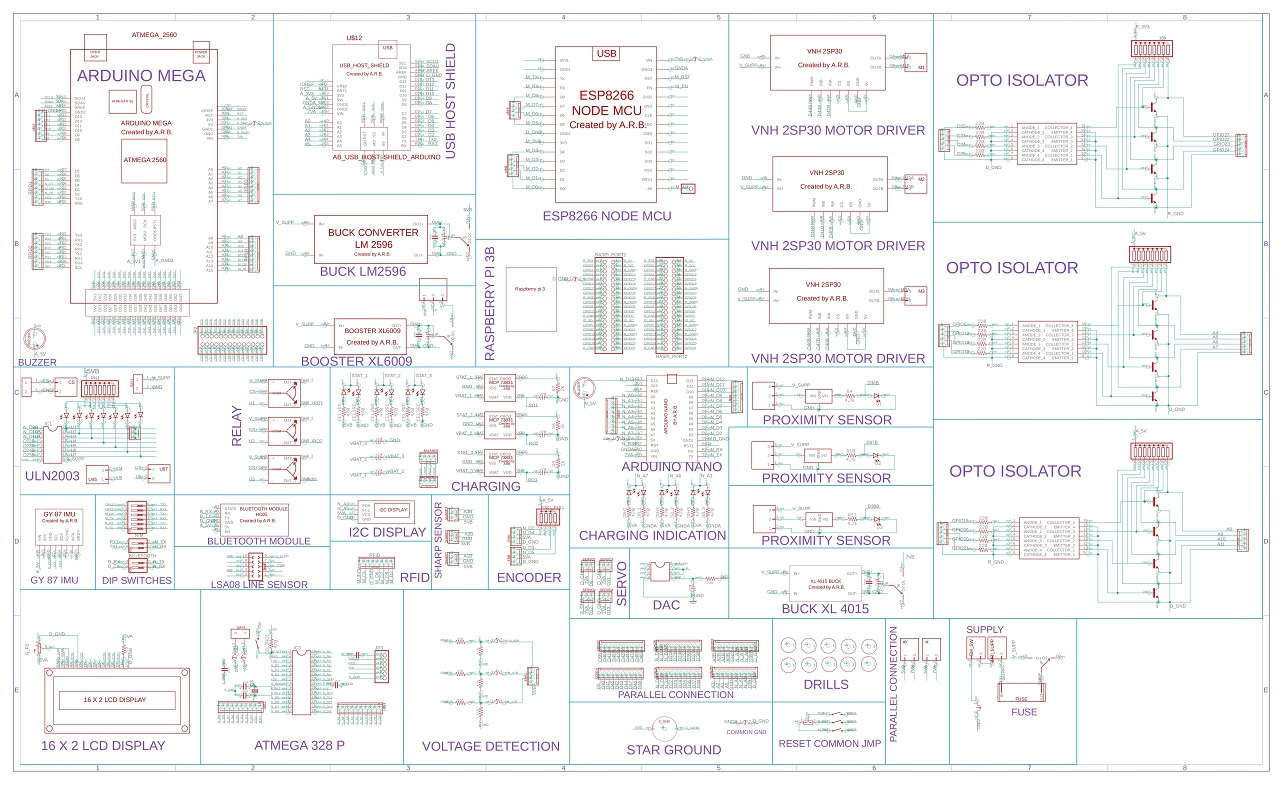
\includegraphics[width = 13cm]{project/images/schematic.jpg}
    \caption{Schematic}
    \end{figure}

    \item \textbf{Board Routing}
    \vspace{-0.5cm}
    \paragraph{} Routing shows the all the tracks on the board. Red tracks indicate top copper and blue tracks indicate bottom copper as shown in Fig. \ref{boardrouting}. Adequate trace width is necessary to ensure the desired amount of current can be transported without overheating and damaging your board. 

    \begin{figure}[H]
    \centering
    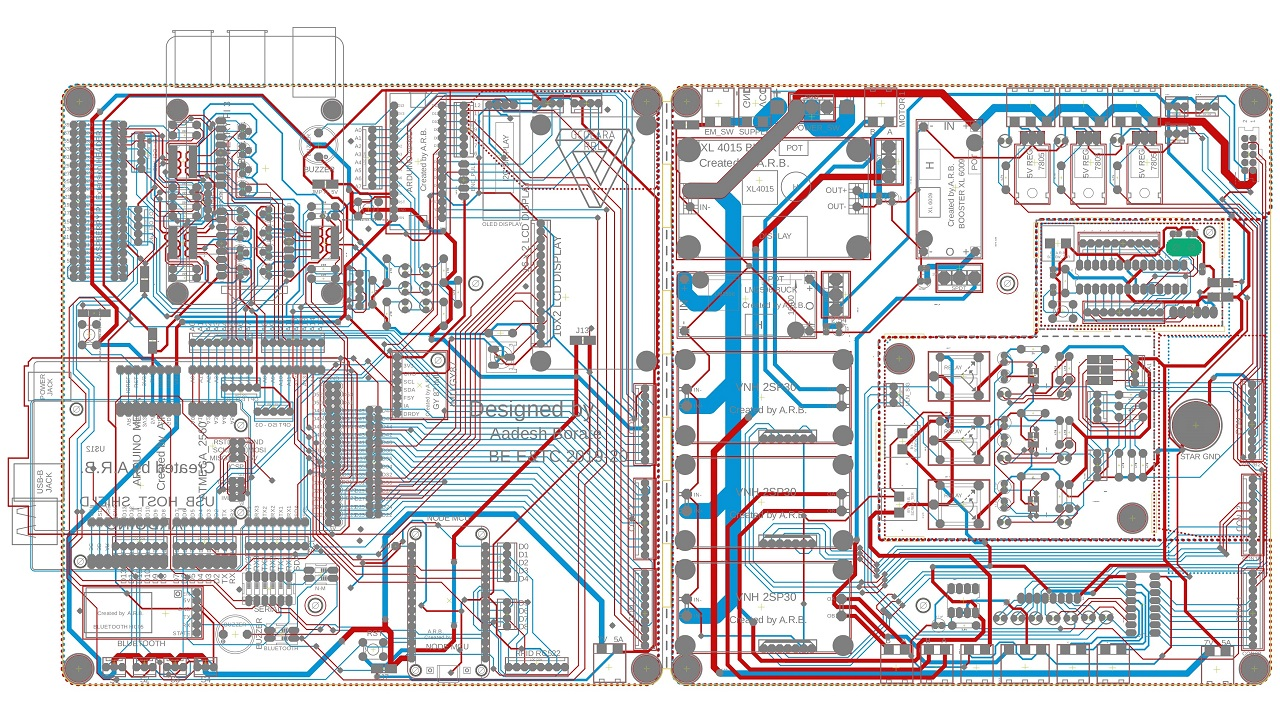
\includegraphics[width = 13cm]{project/images/board_routing_resized.jpg}
    \caption{Board Routing} \label{boardrouting}
    \end{figure}
    
    \item \textbf{PCB Top Side}
    \vspace{-0.5cm}
    \paragraph{} Fig. \ref{Top View} shows the top view of the board in Autodesk Eagle Software.

    \begin{figure}[H]
    \centering
    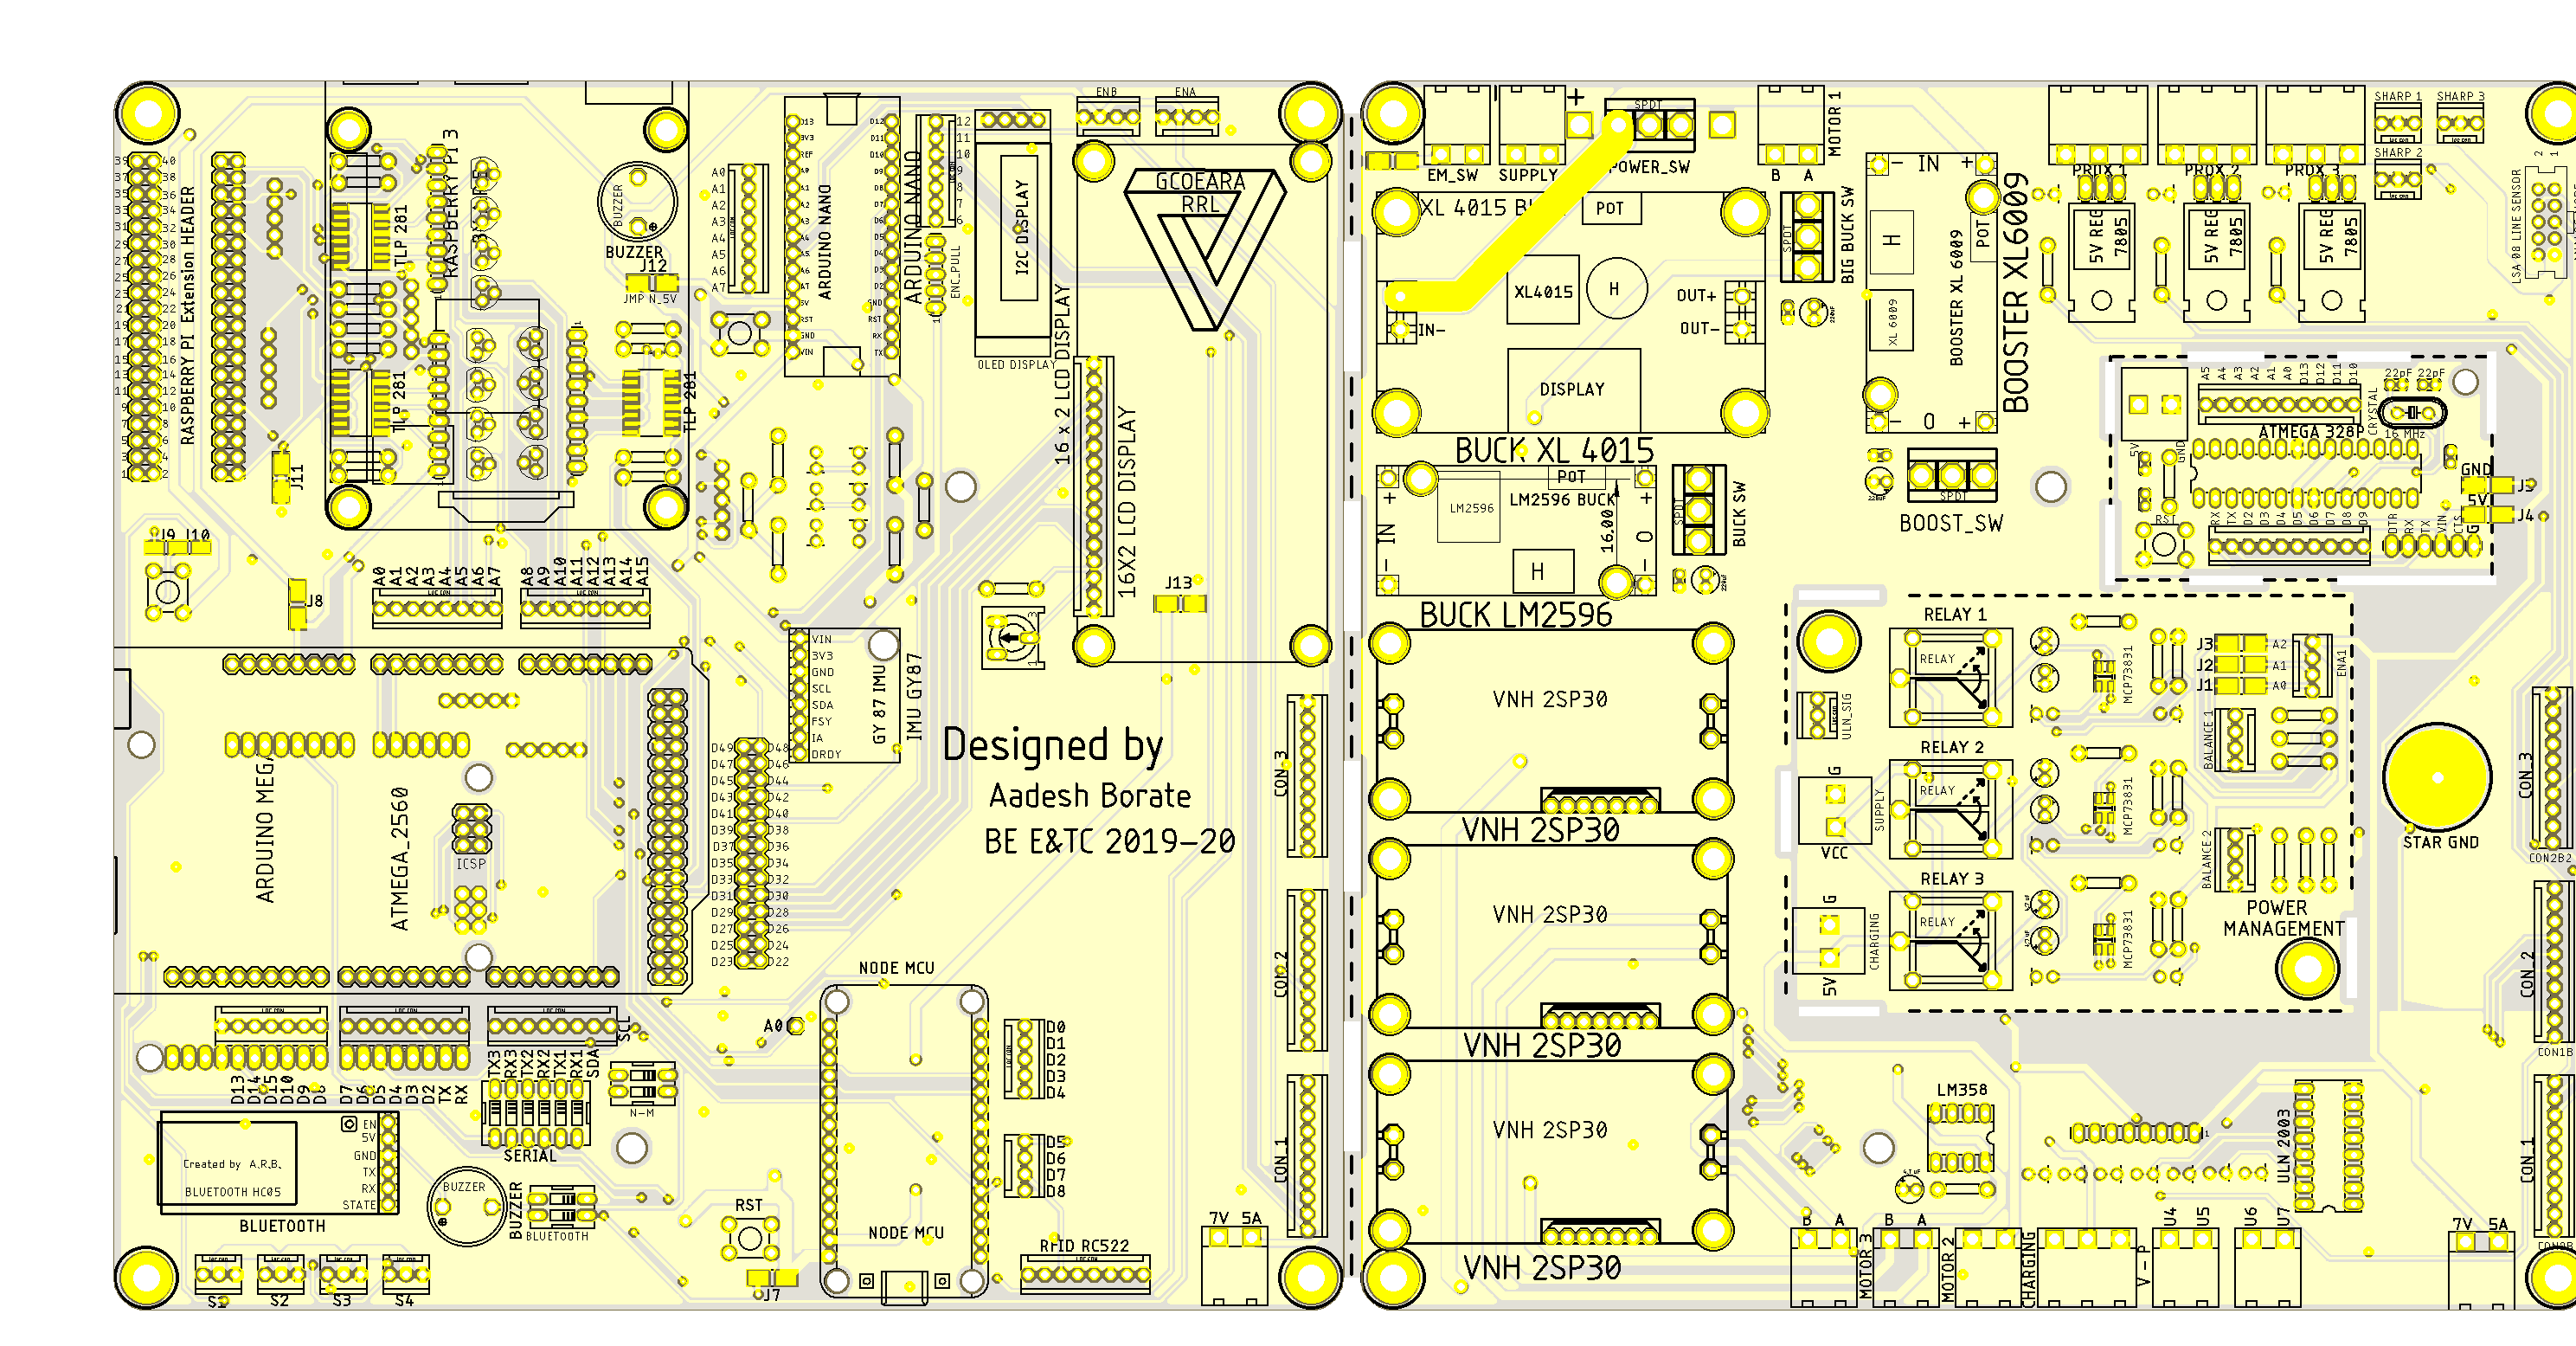
\includegraphics[width = 13cm]{project/images/top_view.png}
    \caption{Top View} \label{Top View}
    \end{figure}
    
    \item \textbf{Printed PCB}
    \vspace{-0.5cm}
    \paragraph{} Fig. \ref{Printed PCB} shows the PCB which is manufactured from Lion Circuits. 

    \begin{figure}[H]
    \centering
    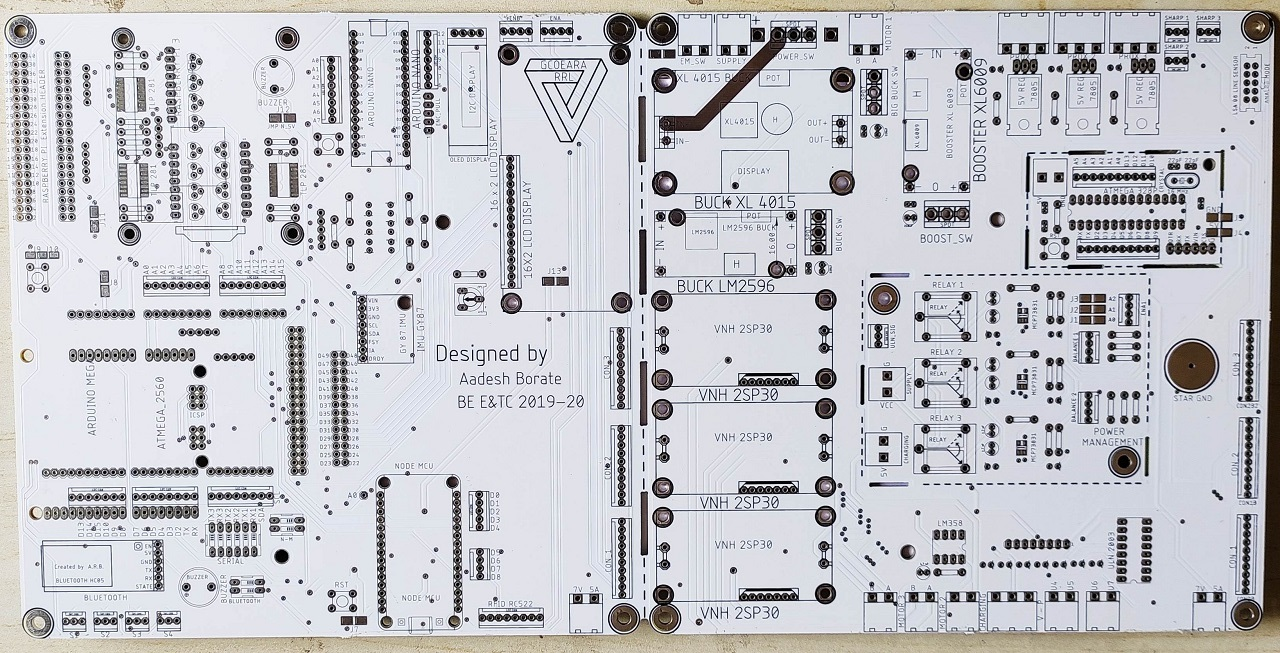
\includegraphics[width = 13cm]{project/images/actual_pcb_resized.jpg}
    \caption{Printed PCB} \label{Printed PCB}
    \end{figure}

\end{itemize}

\newpage

\subsection{Mobile Robotics}
\paragraph{}This module contains the navigation of AGV, tasks done by AGV like pick and place using robotic arm, it's remote access, etc.

\begin{itemize}[wide, labelwidth=!, labelindent=0pt]
    \item \textbf{Robotic Arm}
    \vspace{-0.5cm}
    \paragraph{}Robotic Arm present on the AGV is used for the pick and place of the boxes from one point to another. It is a servo based.
    
    We have used one Servo for two motion i.e. grabbing motion and picking motion. It means one Servo based arm has Two Degree of Freedom.
    
    Linkages of Side Arm are 3D printed as per our measurement.
    
    \begin{figure}[H]
    \centering
    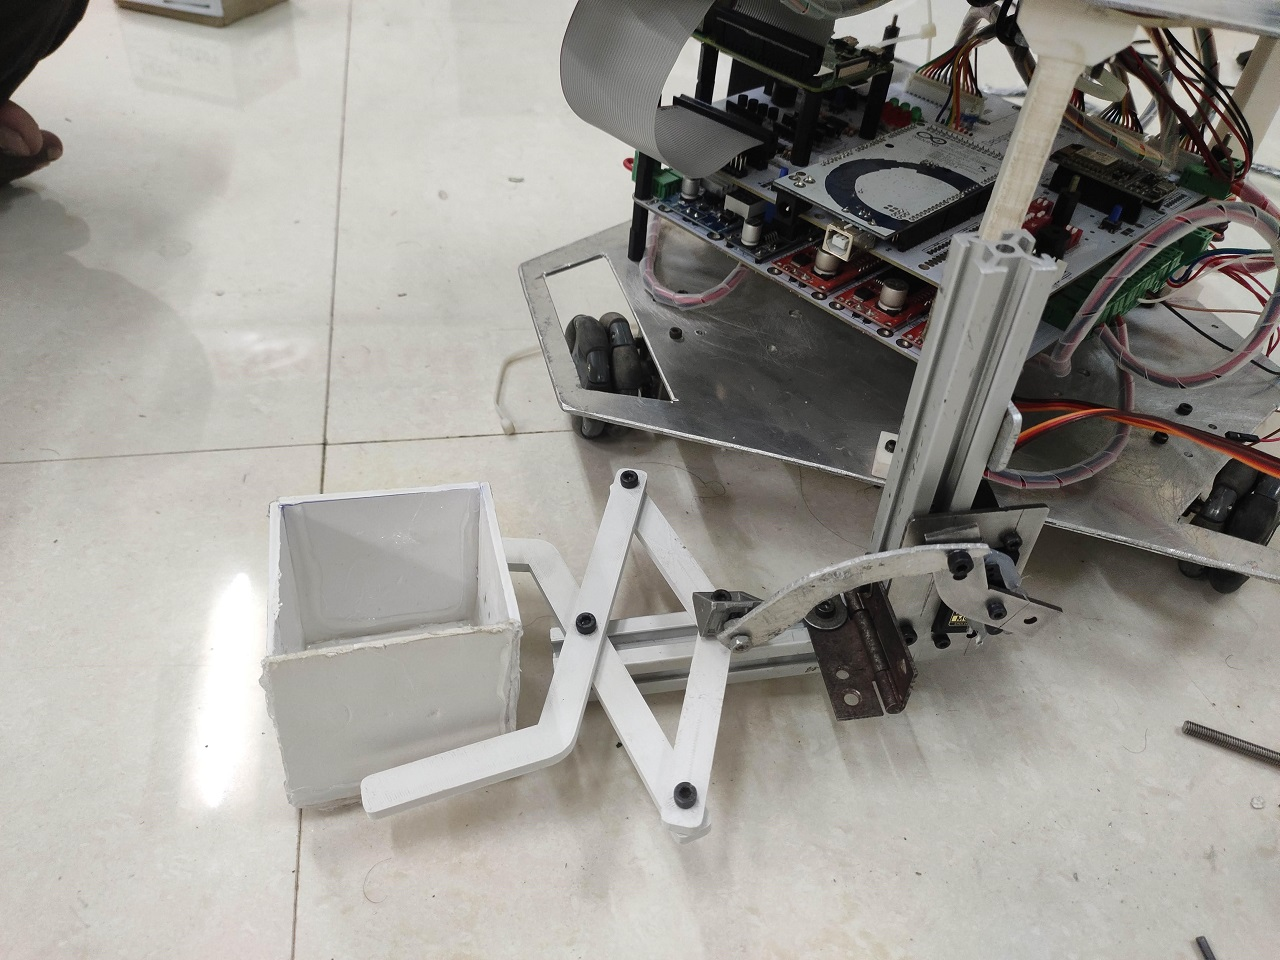
\includegraphics[width = 13cm]{project/images/side_arm.jpg}
    \caption{Side Arm}
    \end{figure}
    
    \newpage
    
    \item \textbf{Remote Access}
    \vspace{-0.5cm}
    \paragraph{}The AGV can be remotely accessed using the WiFi, using the ESP8266 board present on it. A web based graphical user interface is also designed for providing start and destination points for A* algorithm implementation.
    
    \begin{figure}[H]
    \centering
    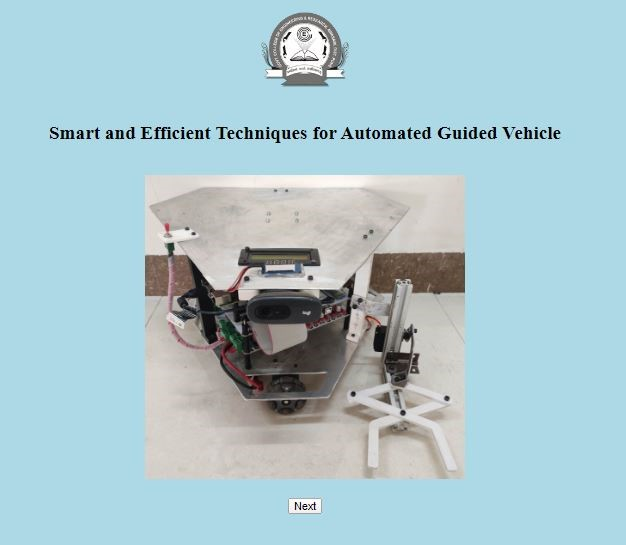
\includegraphics[width = 10cm]{project/images/gui_page1.jpg}
    \caption{GUI page 1}
    \end{figure}
    
    
    \begin{figure}[H]
    \centering
    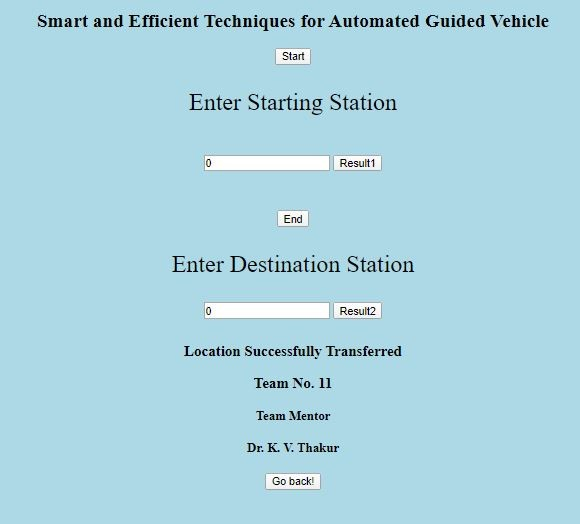
\includegraphics[width = 10cm]{project/images/gui_page2.jpg}
    \caption{GUI page 2}
    \end{figure}
    
    \newpage
    
    \item \textbf{Holonomic motion using Inverse Kinematics}
    \vspace{-0.5cm}
    \paragraph{}Holonomic motion is the motion of the robot keeping the head constant. Navigation of AGV is done automatically by taking feedback of line, QR codes and the IMU. Inverse kinematic equations are used to calculate direction of motion of the AGV.
    
    \begin{figure}[H]
    \centering
    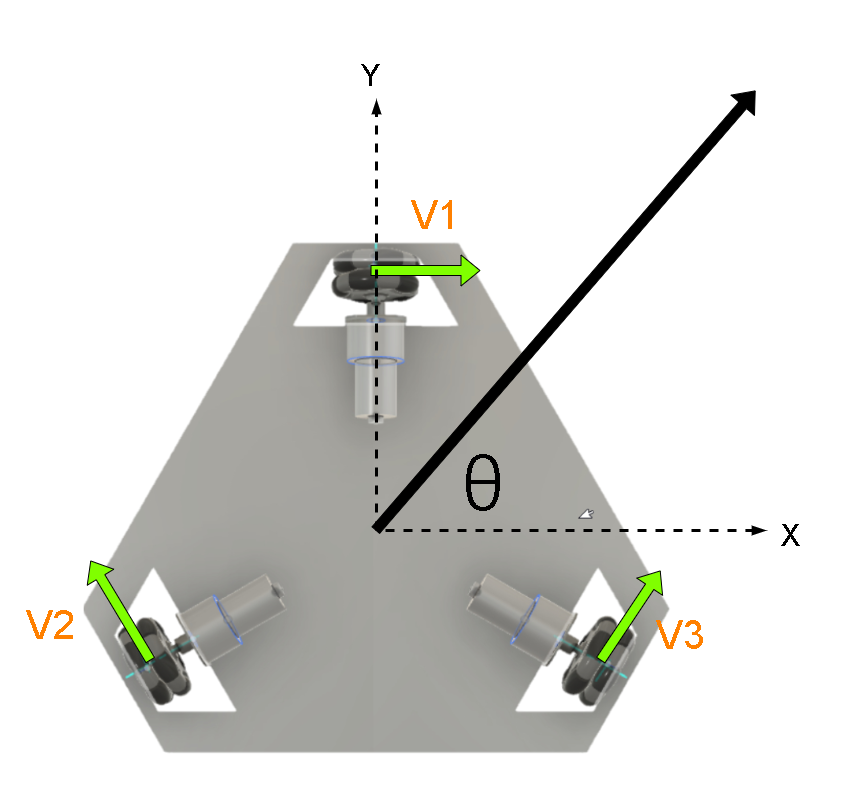
\includegraphics[width = 13cm]{project/images/holonomic.png}
    \caption{Wheel's Direction}
    \end{figure}
    
    $$V_x = V * cos(\theta)$$
    $$V_y = V * sin(\theta)$$
    
    $$V_1 = cos(0)*V_x + sin(0)*V_y$$
    $$V_1 = cos(120)*V_x + sin(120)*V_y$$
    $$V_1 = cos(60)*V_x + sin(60)*V_y$$

\end{itemize}

\newpage
\subsection{Machine Vision}

\paragraph{}Machine vision (MV) is the technology and methods used to provide imaging-based automatic inspection and analysis for such applications as automatic inspection, process control, and robot guidance, usually in industry. Machine vision refers to many technologies, software and hardware products, integrated systems, actions, methods and expertise. Machine vision as a systems engineering discipline can be considered distinct from computer vision, a form of computer science. It attempts to integrate existing technologies in new ways and apply them to solve real world problems.\\

MV in our project is accomplished by using OpenCV library and Python language. OpenCV (Open Source Computer Vision Library) is an open source computer vision and machine learning software library. Hardware used is Raspberry Pi 4 Model B.\\

\begin{itemize}[wide, labelwidth=!, labelindent=0pt]
    \item \textbf{Face Recognition}
    \vspace{-0.5cm} 
    \paragraph{} Specially for face recognition we have used Faster RCNN Inception V3 model. We have also tried SSD Mobilenet V2 model. But one is more fast and one is more accurate.\\
    Training image = 268\\
    Testing image = 67\\
    More images more accuracy but beware of overfitting.
    
    \begin{figure}[H]
    \centering
    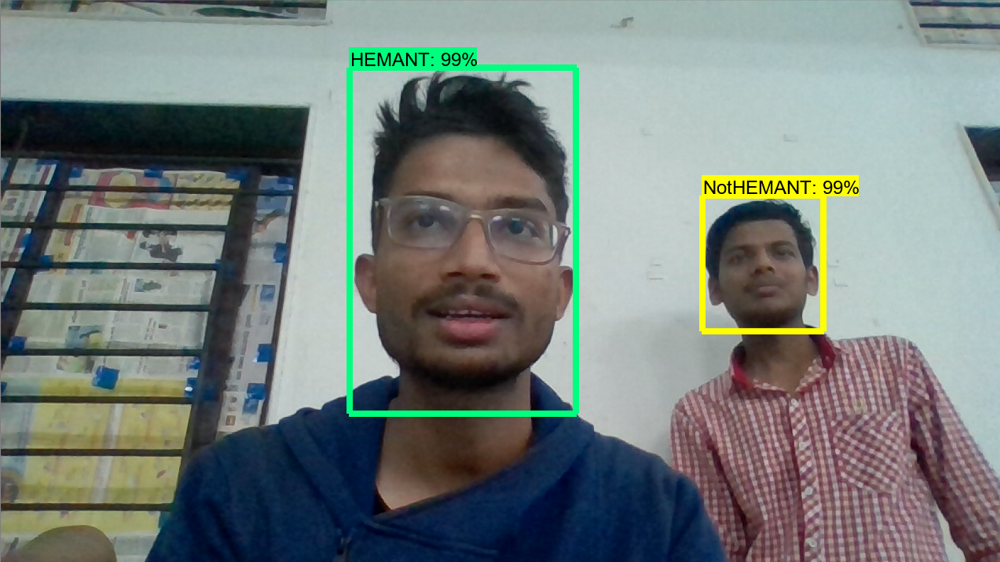
\includegraphics[width = 13cm]{project/images/face_detection.png}
    \caption{Face Recognition}
    \end{figure}

    \item \textbf{Line Detection and Angle Estimation}
    \vspace{-0.5cm}
    \paragraph{} Line detection helps in estimating angle. The various things used for detection of line are given below:
    
    \begin{enumerate}
        \item Gray Level Thresholding
        \item Area Thresholding
        \item Edge Detection
        \item Hough Line Transform
    \end{enumerate}
    
    \begin{figure}[H]
    \centering
    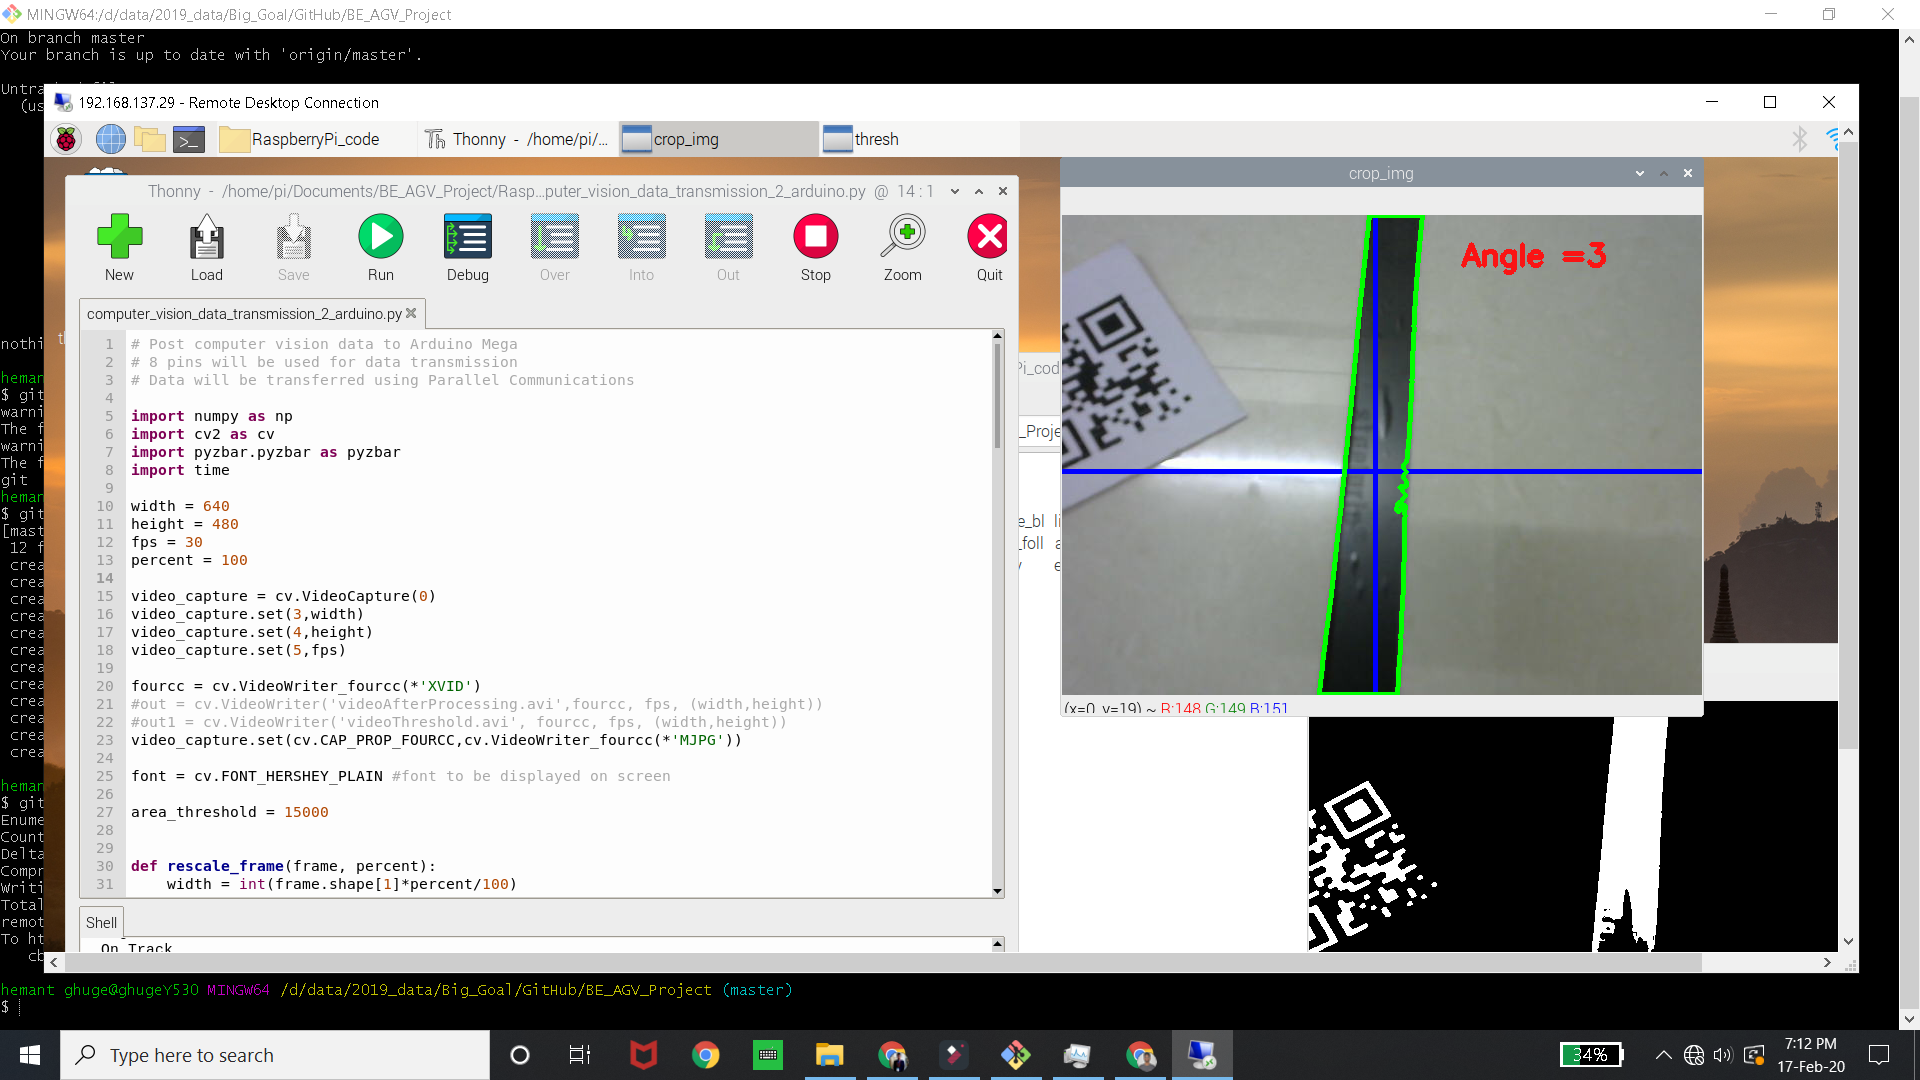
\includegraphics[width = 14cm]{project/images/angle_estimation.png}
    \caption{Line detection and Angle estimation}
    \end{figure}
    
    \item \textbf{QR code scanning}

    \begin{figure}[H]
    \centering
    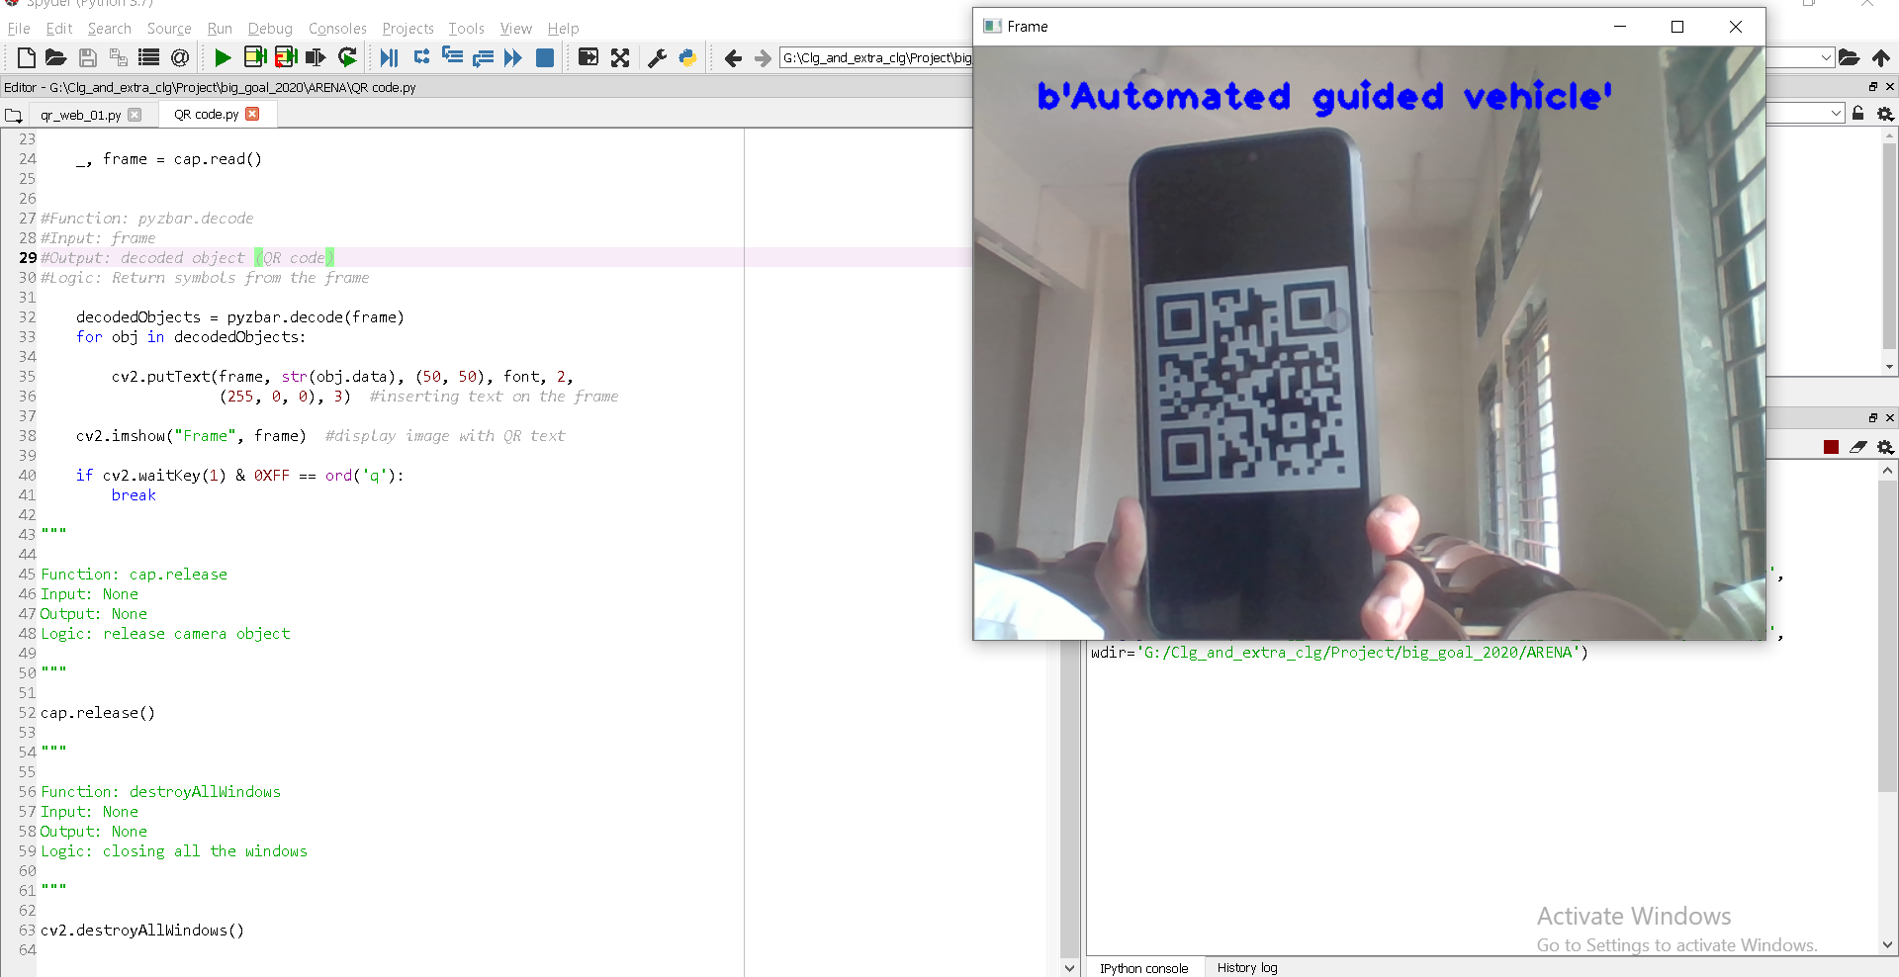
\includegraphics[width = 14cm]{project/images/qr_code_detection.png}
    \caption{QR Code Detection}
    \end{figure}
        
    \item \textbf{Integration of ALL}
    
    \begin{figure}[H]
    \centering
    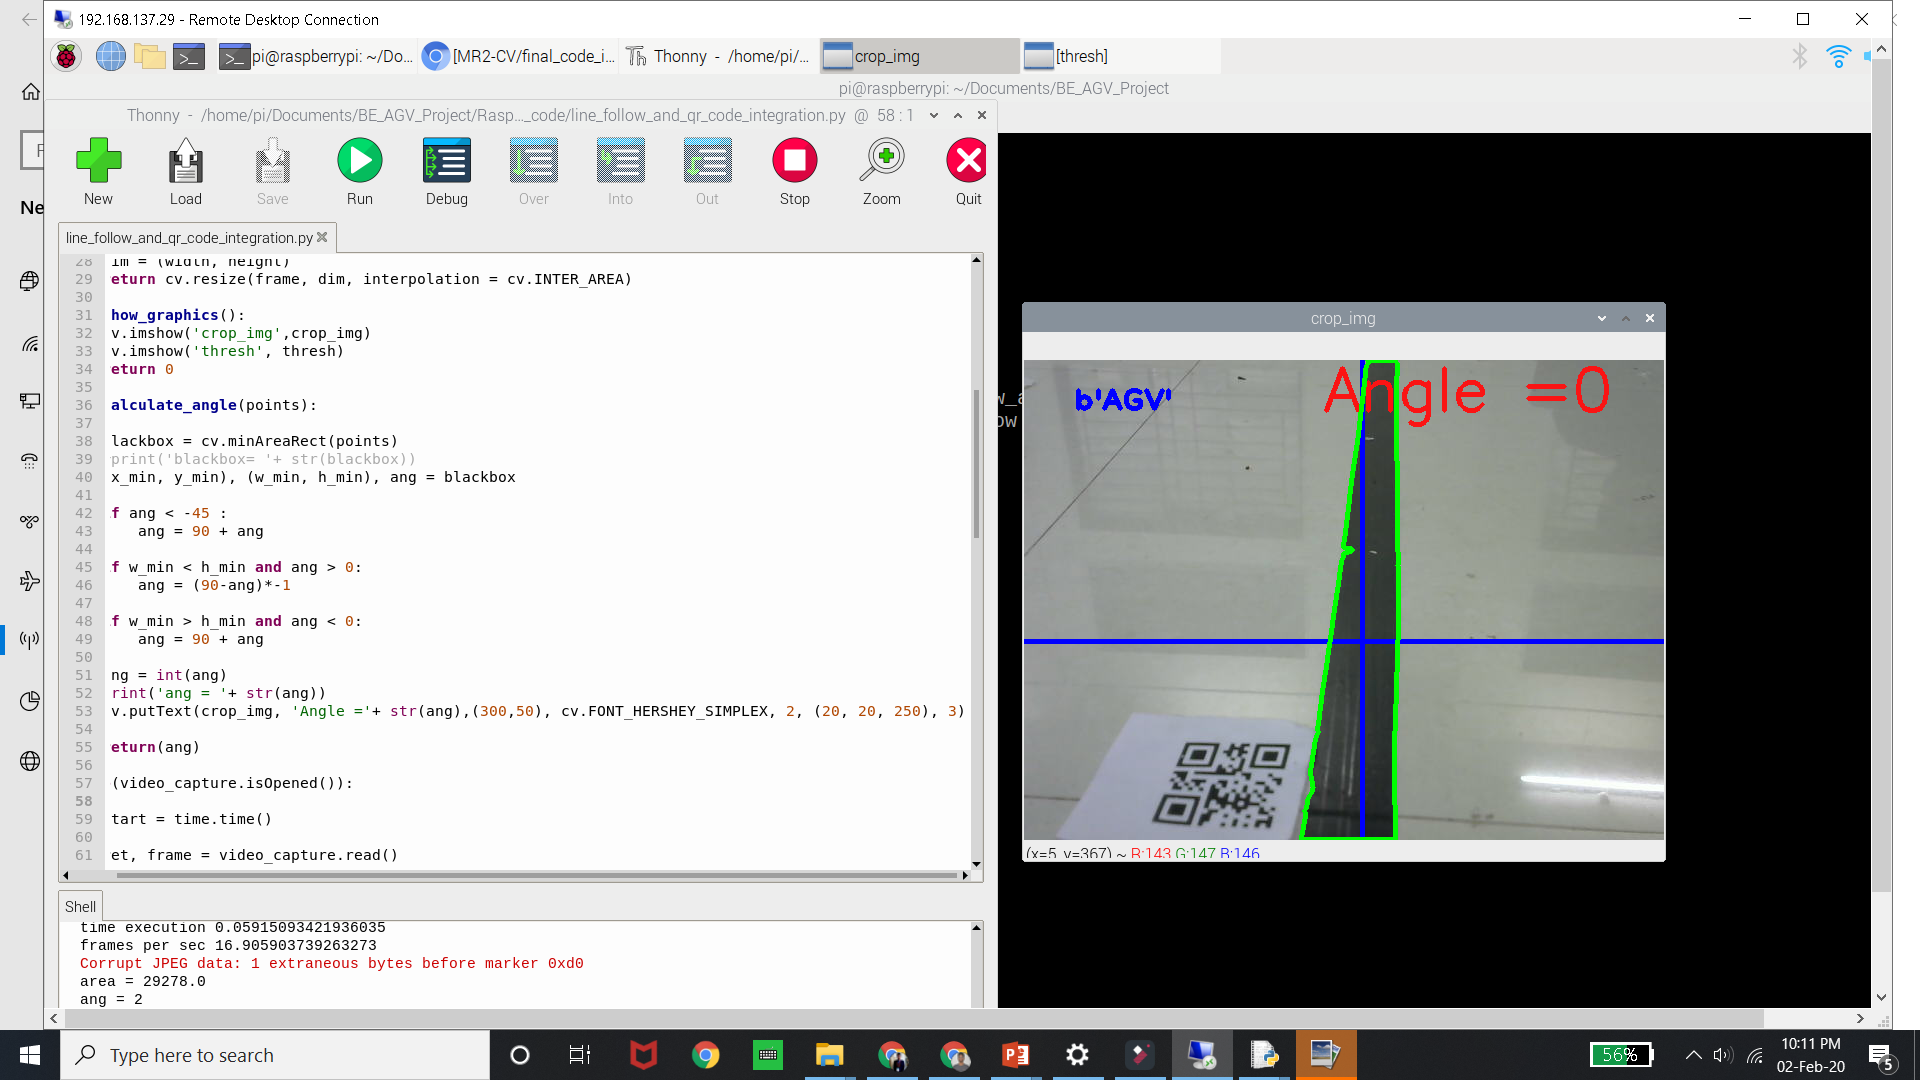
\includegraphics[width = 13cm]{project/images/line_follow_qr_code.png}
    \caption{Line + Angle + QR}
    \end{figure}

\end{itemize}

\subsection{Power Management}

Power management is a computing device feature that allows users to control the amount of electrical power consumed by an underlying device, with minimal impact on performance. It enables the switching of devices in various power modes, each with different power usage characteristics related to device performance.

\begin{itemize}[wide, labelwidth=!, labelindent=0pt]
    \item \textbf{Voltage estimation}
    \vspace{-0.5cm}
    \paragraph{} Voltage estimation helps in detecting low voltage.
    \begin{figure}[h]
    \subfloat[Subfigure 1 list of figures text][Cell 1]{
    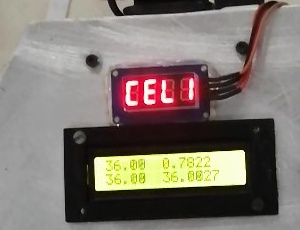
\includegraphics[width=0.25\textwidth]{project/images/cell1crop.jpg}
    \label{all:cell1}}
    \subfloat[Subfigure 2 list of figures text][Cell 1 Voltage]{
    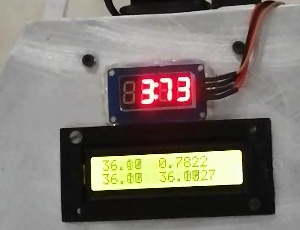
\includegraphics[width=0.25\textwidth]{project/images/cell1valuecrop.jpg}
    \label{all:cell1value}}
    \subfloat[Subfigure 3 list of figures text][Cell 2]{
    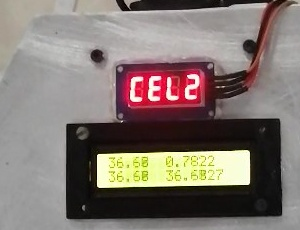
\includegraphics[width=0.25\textwidth]{project/images/cell2crop.jpg}
    \label{all:cell2}}
    \subfloat[Subfigure 4 list of figures text][Cell 2 Voltage]{
    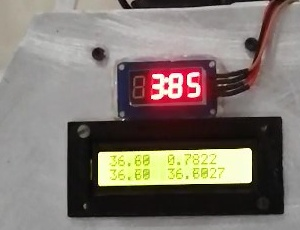
\includegraphics[width=0.25\textwidth]{project/images/cell2valuecrop.jpg}
    \label{all:cell2value}}
    \qquad
    \subfloat[Subfigure 5 list of figures text][Cell 3]{
    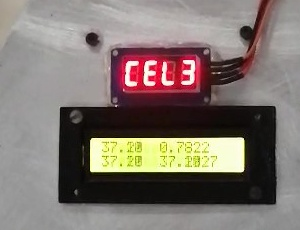
\includegraphics[width=0.25\textwidth]{project/images/cell3crop.jpg}
    \label{all:cell3}}
    \subfloat[Subfigure 6 list of figures text][Cell 3 Voltage]{
    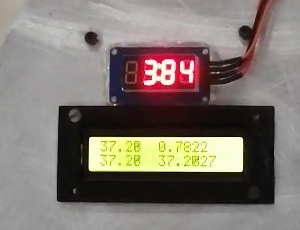
\includegraphics[width=0.25\textwidth]{project/images/cell3valuecrop.jpg}
    \label{all:cell3value}}
    \subfloat[Subfigure 7 list of figures text][All]{
    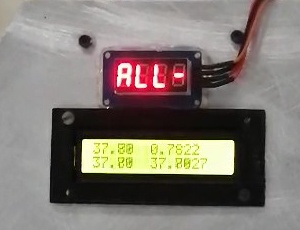
\includegraphics[width=0.25\textwidth]{project/images/allcrop.jpg}
    \label{all:total}}
    \subfloat[Subfigure 8 list of figures text][Total/All Voltage]{
    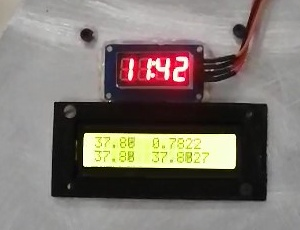
\includegraphics[width=0.25\textwidth]{project/images/allvaluecrop.jpg}
    \label{all:totalvalue}}
    \caption{Voltage estimation of each cell}
    \label{all:global}
    \end{figure}

\end{itemize}

\newpage
\subsection{Path Planning/Control System}

\begin{itemize}[wide, labelwidth=!, labelindent=0pt]
    \item \textbf{Path Planning Algorithm}
    \vspace{-0.5cm} 
    \paragraph{} Finding the shortest path between start point and destination is important to increase speed and efficiency of the work. We have used A* Algorithm as our Path Planning Algorithm. A* algorithm finds shortest path based on the cost to reach the nodes as well as the heuristic function. A heuristic function decides which path should be chosen from the available alternatives, and the main advantage of it is that it can be defined by user. Thus we can assign the priorities to the node points and we will get our required shortest path.

    \begin{figure}[H]
    \centering
    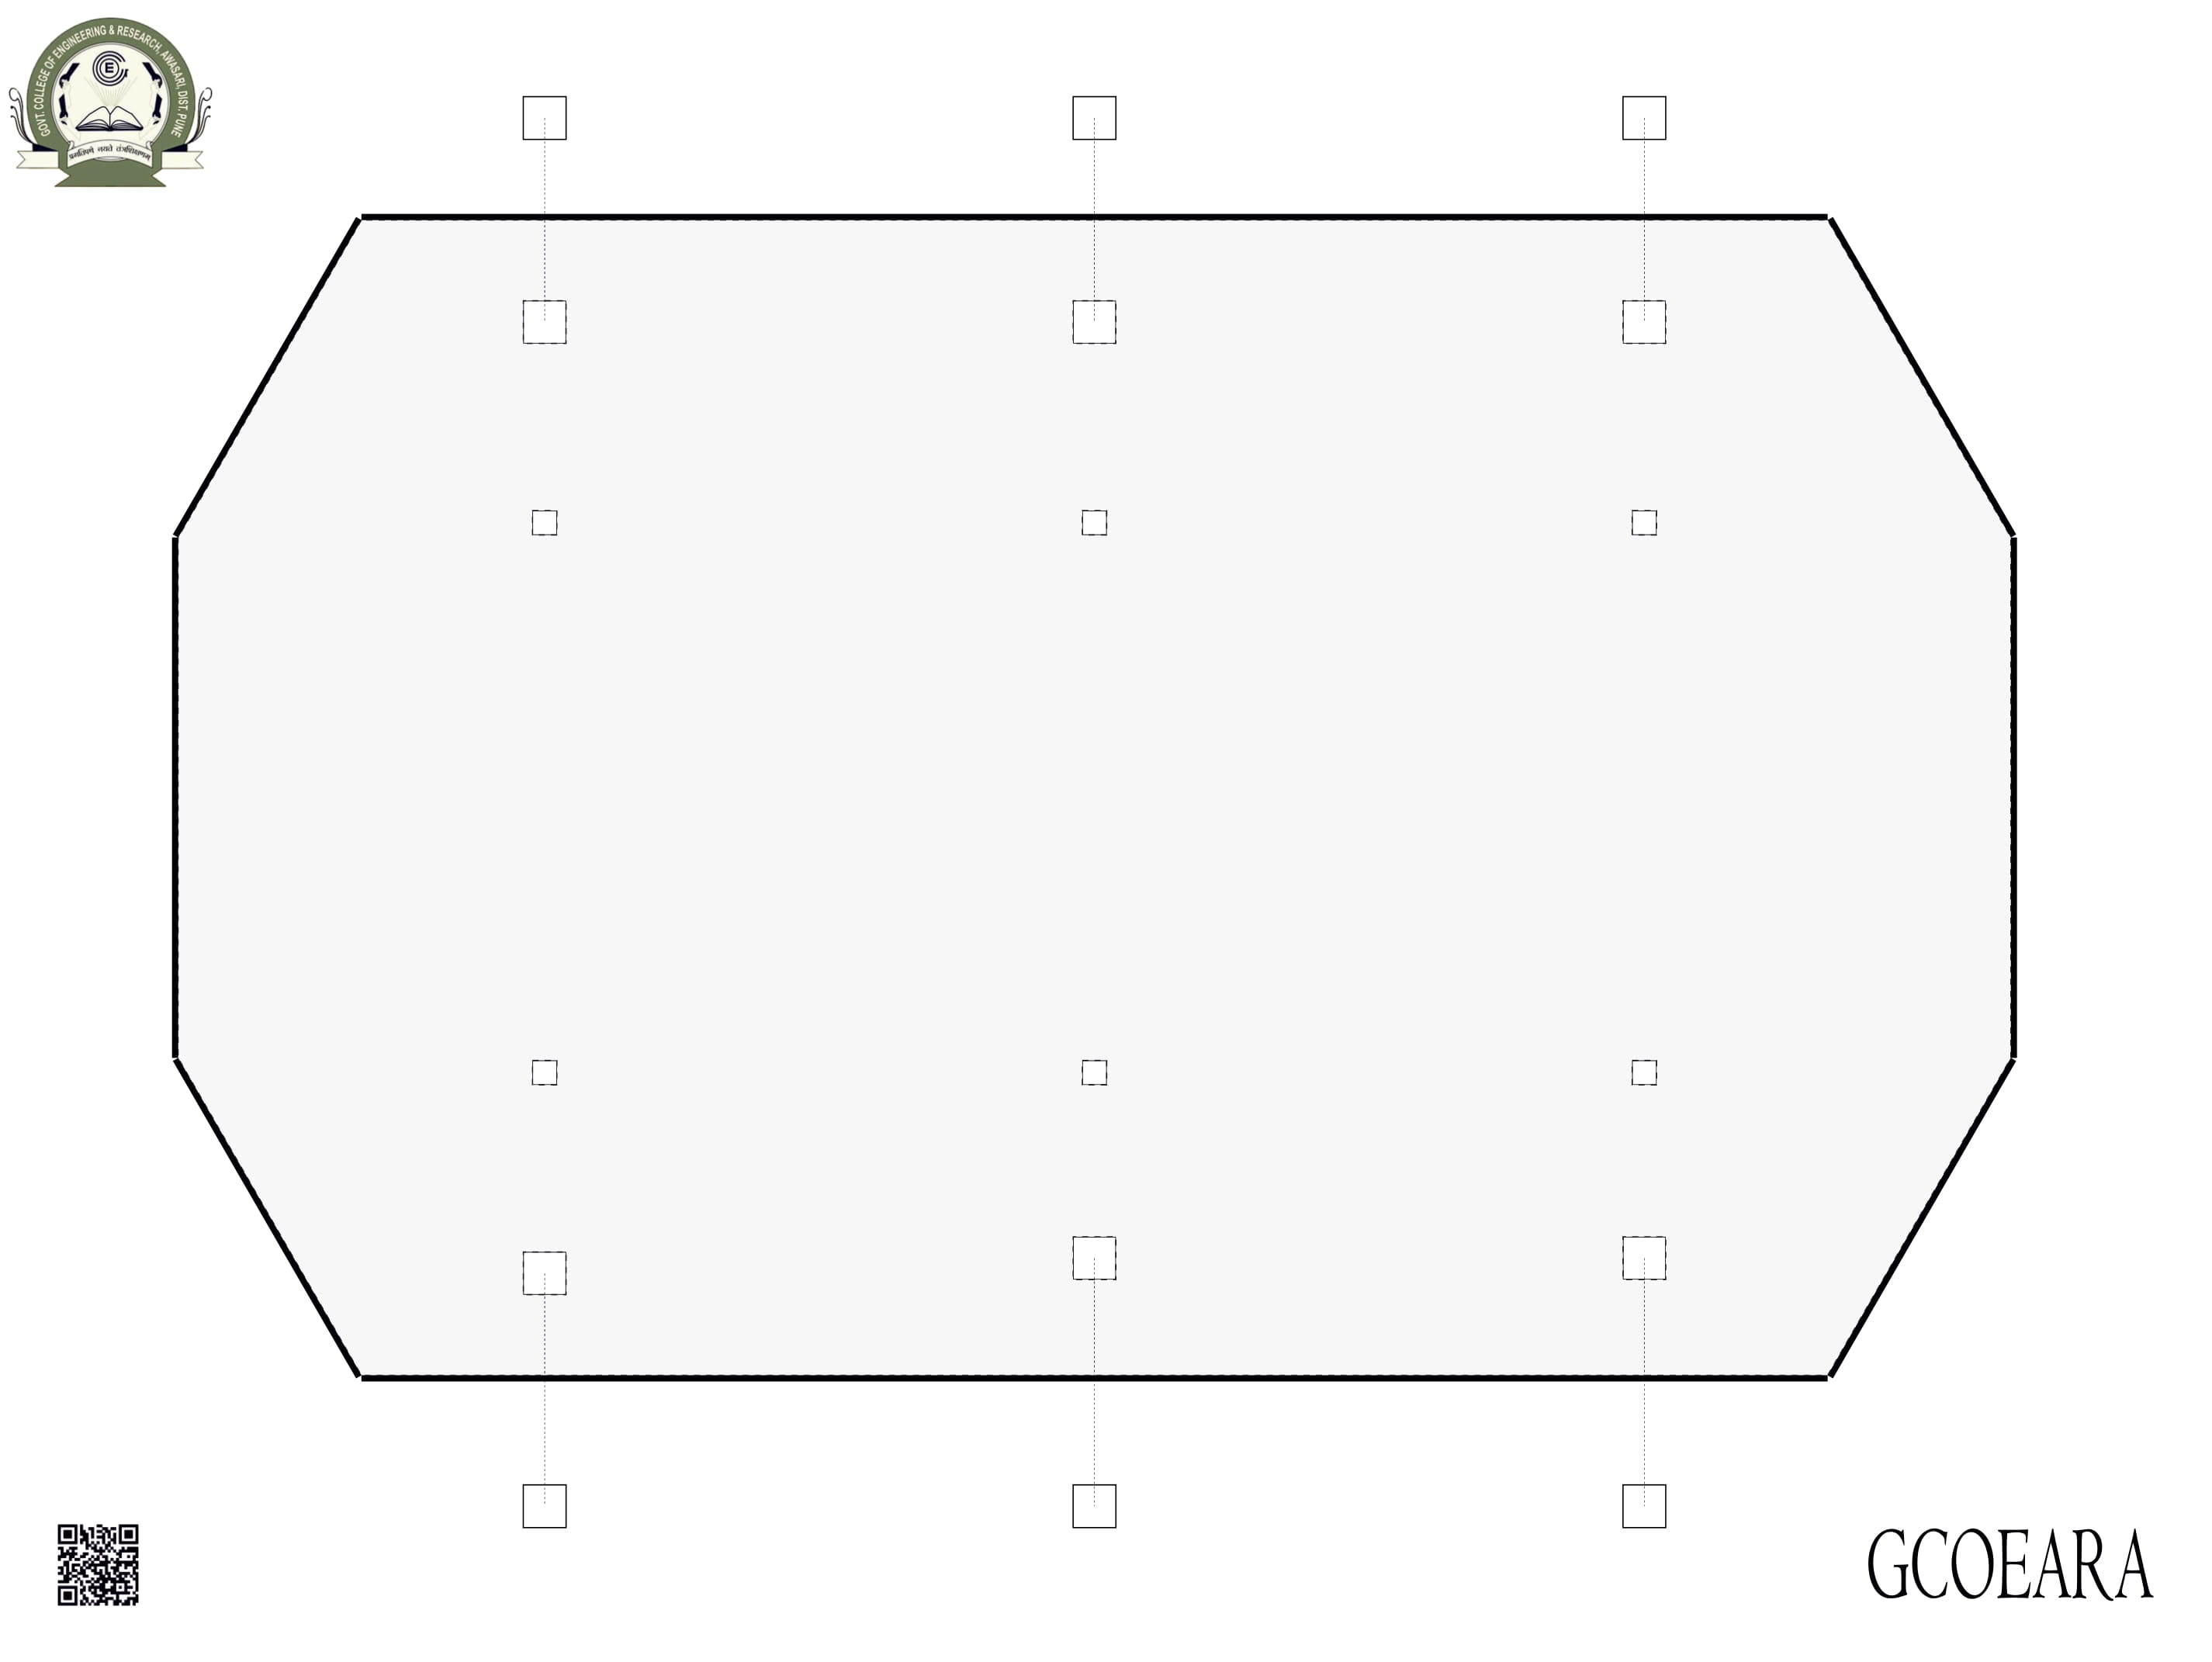
\includegraphics[width = \textwidth]{project/images/arena.jpg}
    \caption{Arena}
    \end{figure}
    
    \begin{itemize}
        \item Size - 362cm * 272cm
        \item Small square - Position of QR code node
        \item Large square - Position of boxes 
        \item Black Line - Line Following Line
    \end{itemize}

    \newpage
    \item \textbf{Control System}
    \vspace{-0.5cm} 
    \paragraph{} As we have discussed the holonomic motion, we need control system for stability.
    
    A control system is a system, which provides the desired response by controlling the output. The following Fig. \ref{cs} shows the simple block diagram of a control system.
    
    \begin{figure}[H]
    \centering
    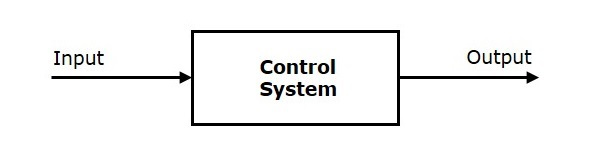
\includegraphics[width = 10cm]{project/images/control_system.jpg}
    \caption{Block Diagram of Control System}\label{cs}
    \end{figure}
    
    Here, the control system is represented by a single block. Since, the output is controlled by varying input, the control system got this name. We will vary this input with some mechanism.
    
     In control system, we use PID controller for head control feature. PID control is a mathematical approach to a broad range of output control scenarios. Whenever a system needs to tune an output based on some input value, PID techniques offer a neat starting point to implement a solution.
    
    \begin{figure}[H]
    \centering
    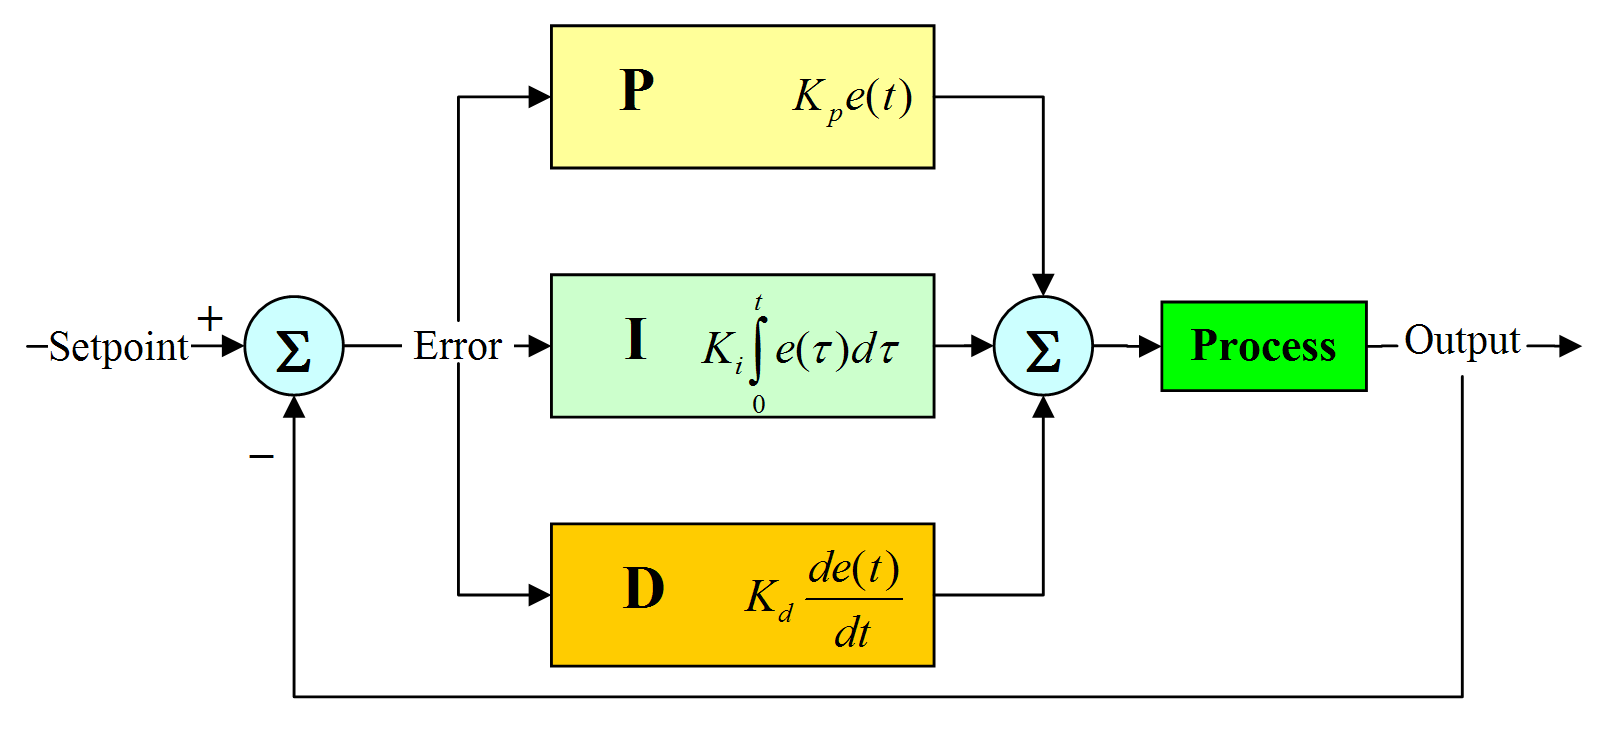
\includegraphics[width = 14cm]{project/images/pid.png}
    \caption{PID controller}
    \end{figure}
    
\end{itemize}

\newpage

\subsection{Embedded System}

\paragraph{} An embedded system is a computer system—a combination of a computer processor, computer memory, and input/output peripheral devices—that has a dedicated function within a larger mechanical or electrical system. Industrial machines, consumer electronics, agricultural and process industry devices, automobiles, medical equipment, cameras, household appliances, airplanes, vending machines and toys, as well as mobile devices, are possible locations for an embedded system.


\begin{figure}[H]
\centering
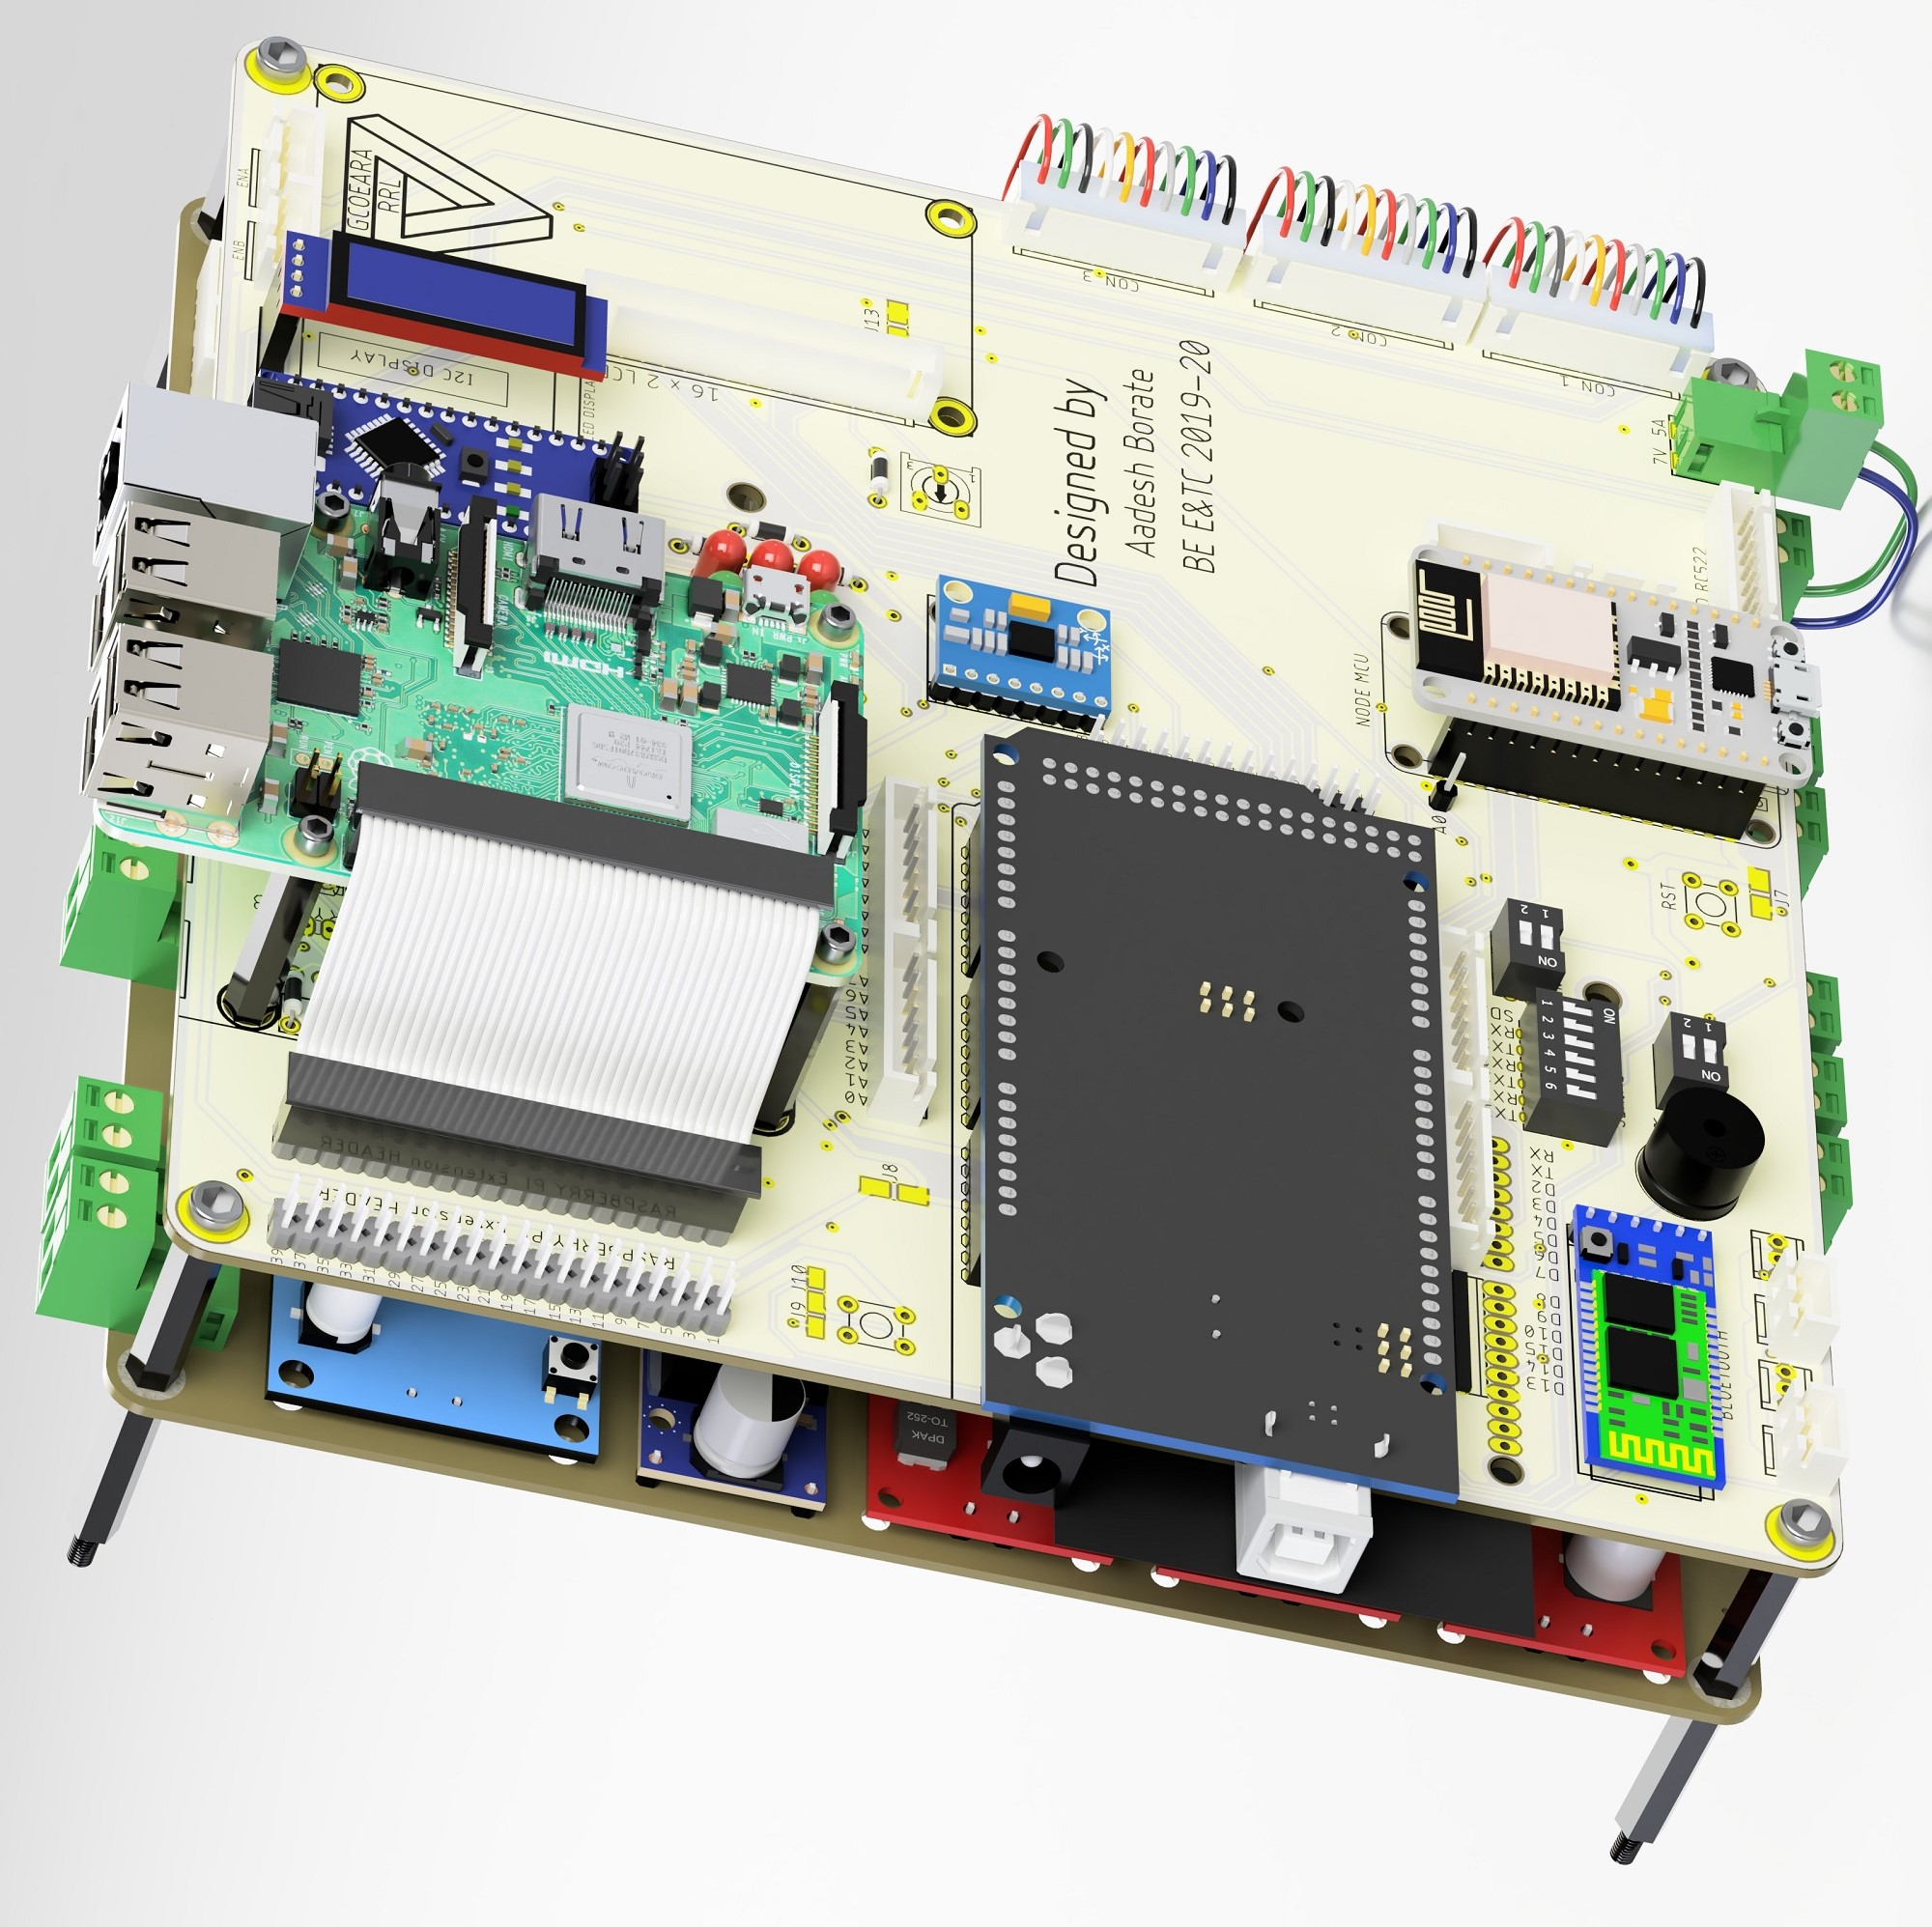
\includegraphics[width = 9cm]{project/images/full circuit 01.jpg}
\caption{PCB with connection 3D Model}
\end{figure}

\begin{figure}[H]
\centering
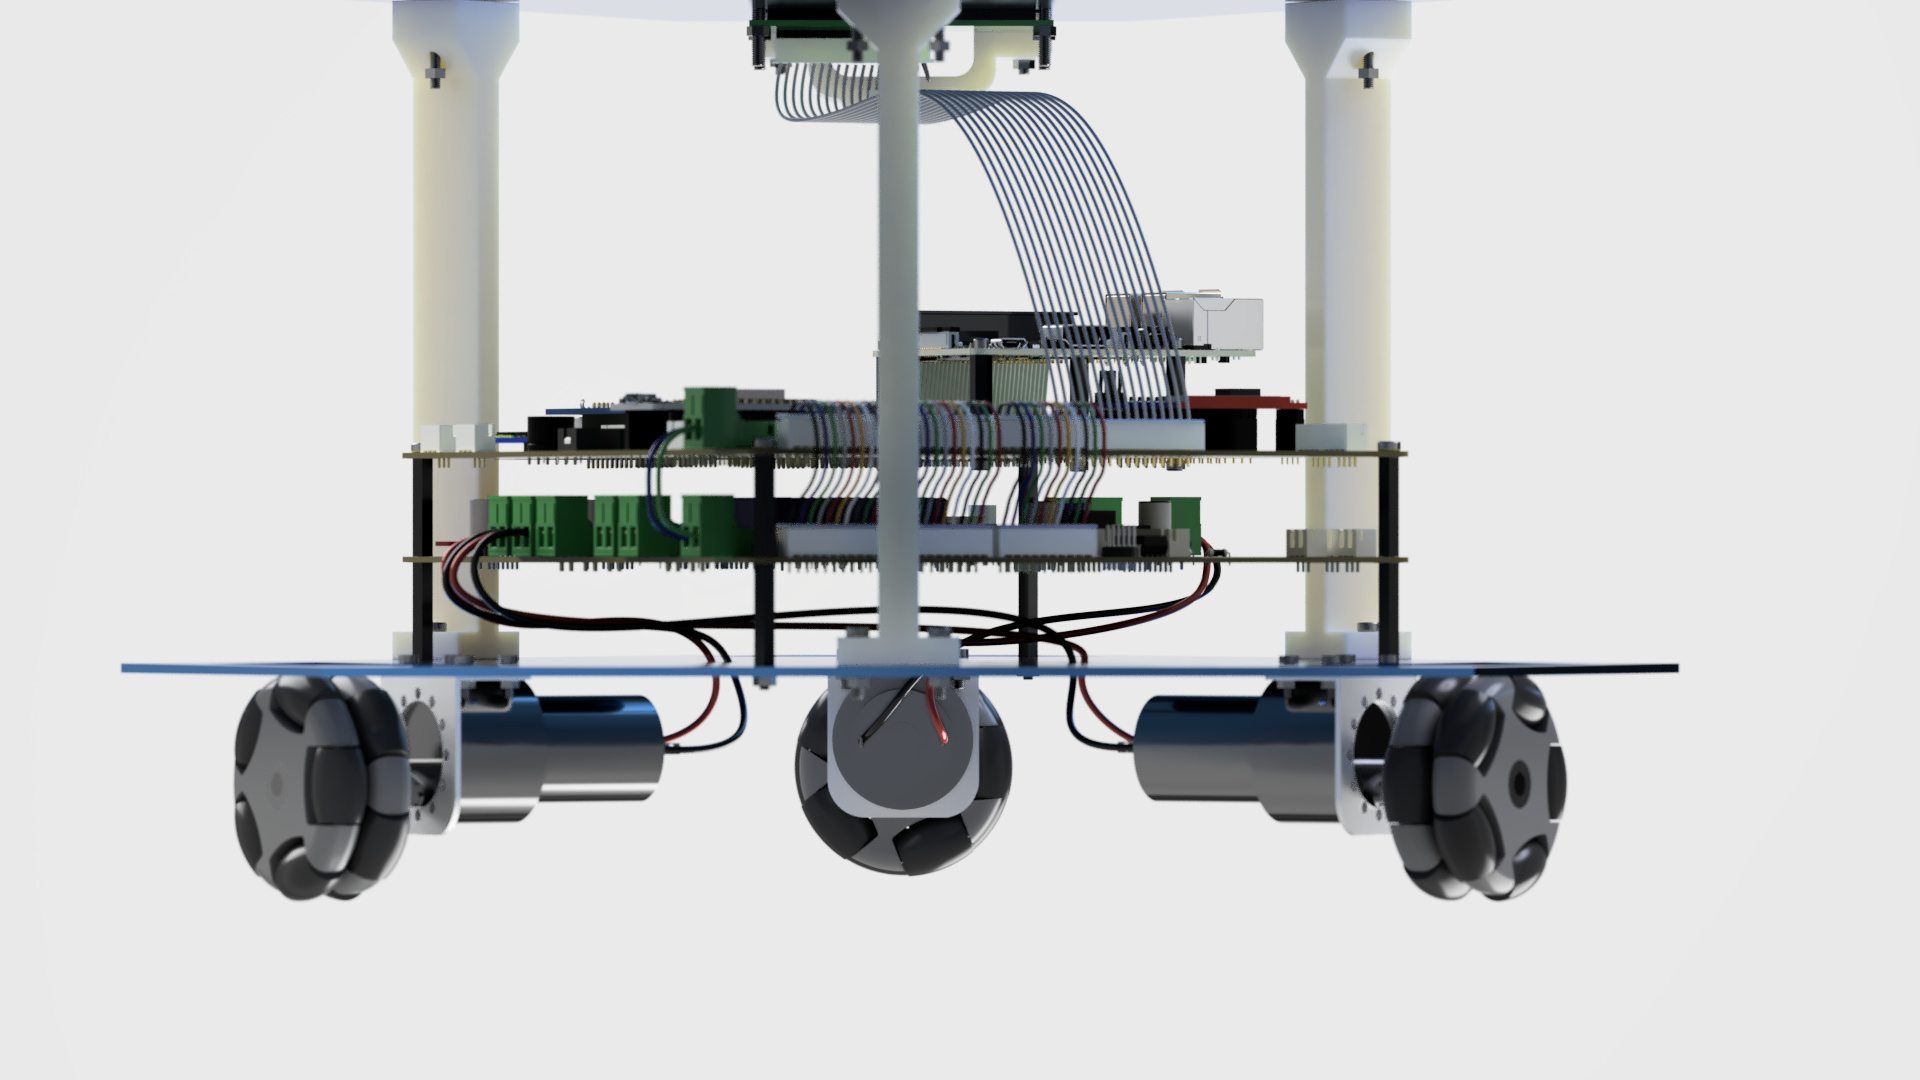
\includegraphics[width = 13cm]{project/images/full circuit 02.jpg}
\caption{AGV 3D Model}
\end{figure}

\newpage
\section{Flowchart}

\begin{figure}[H]
\centering
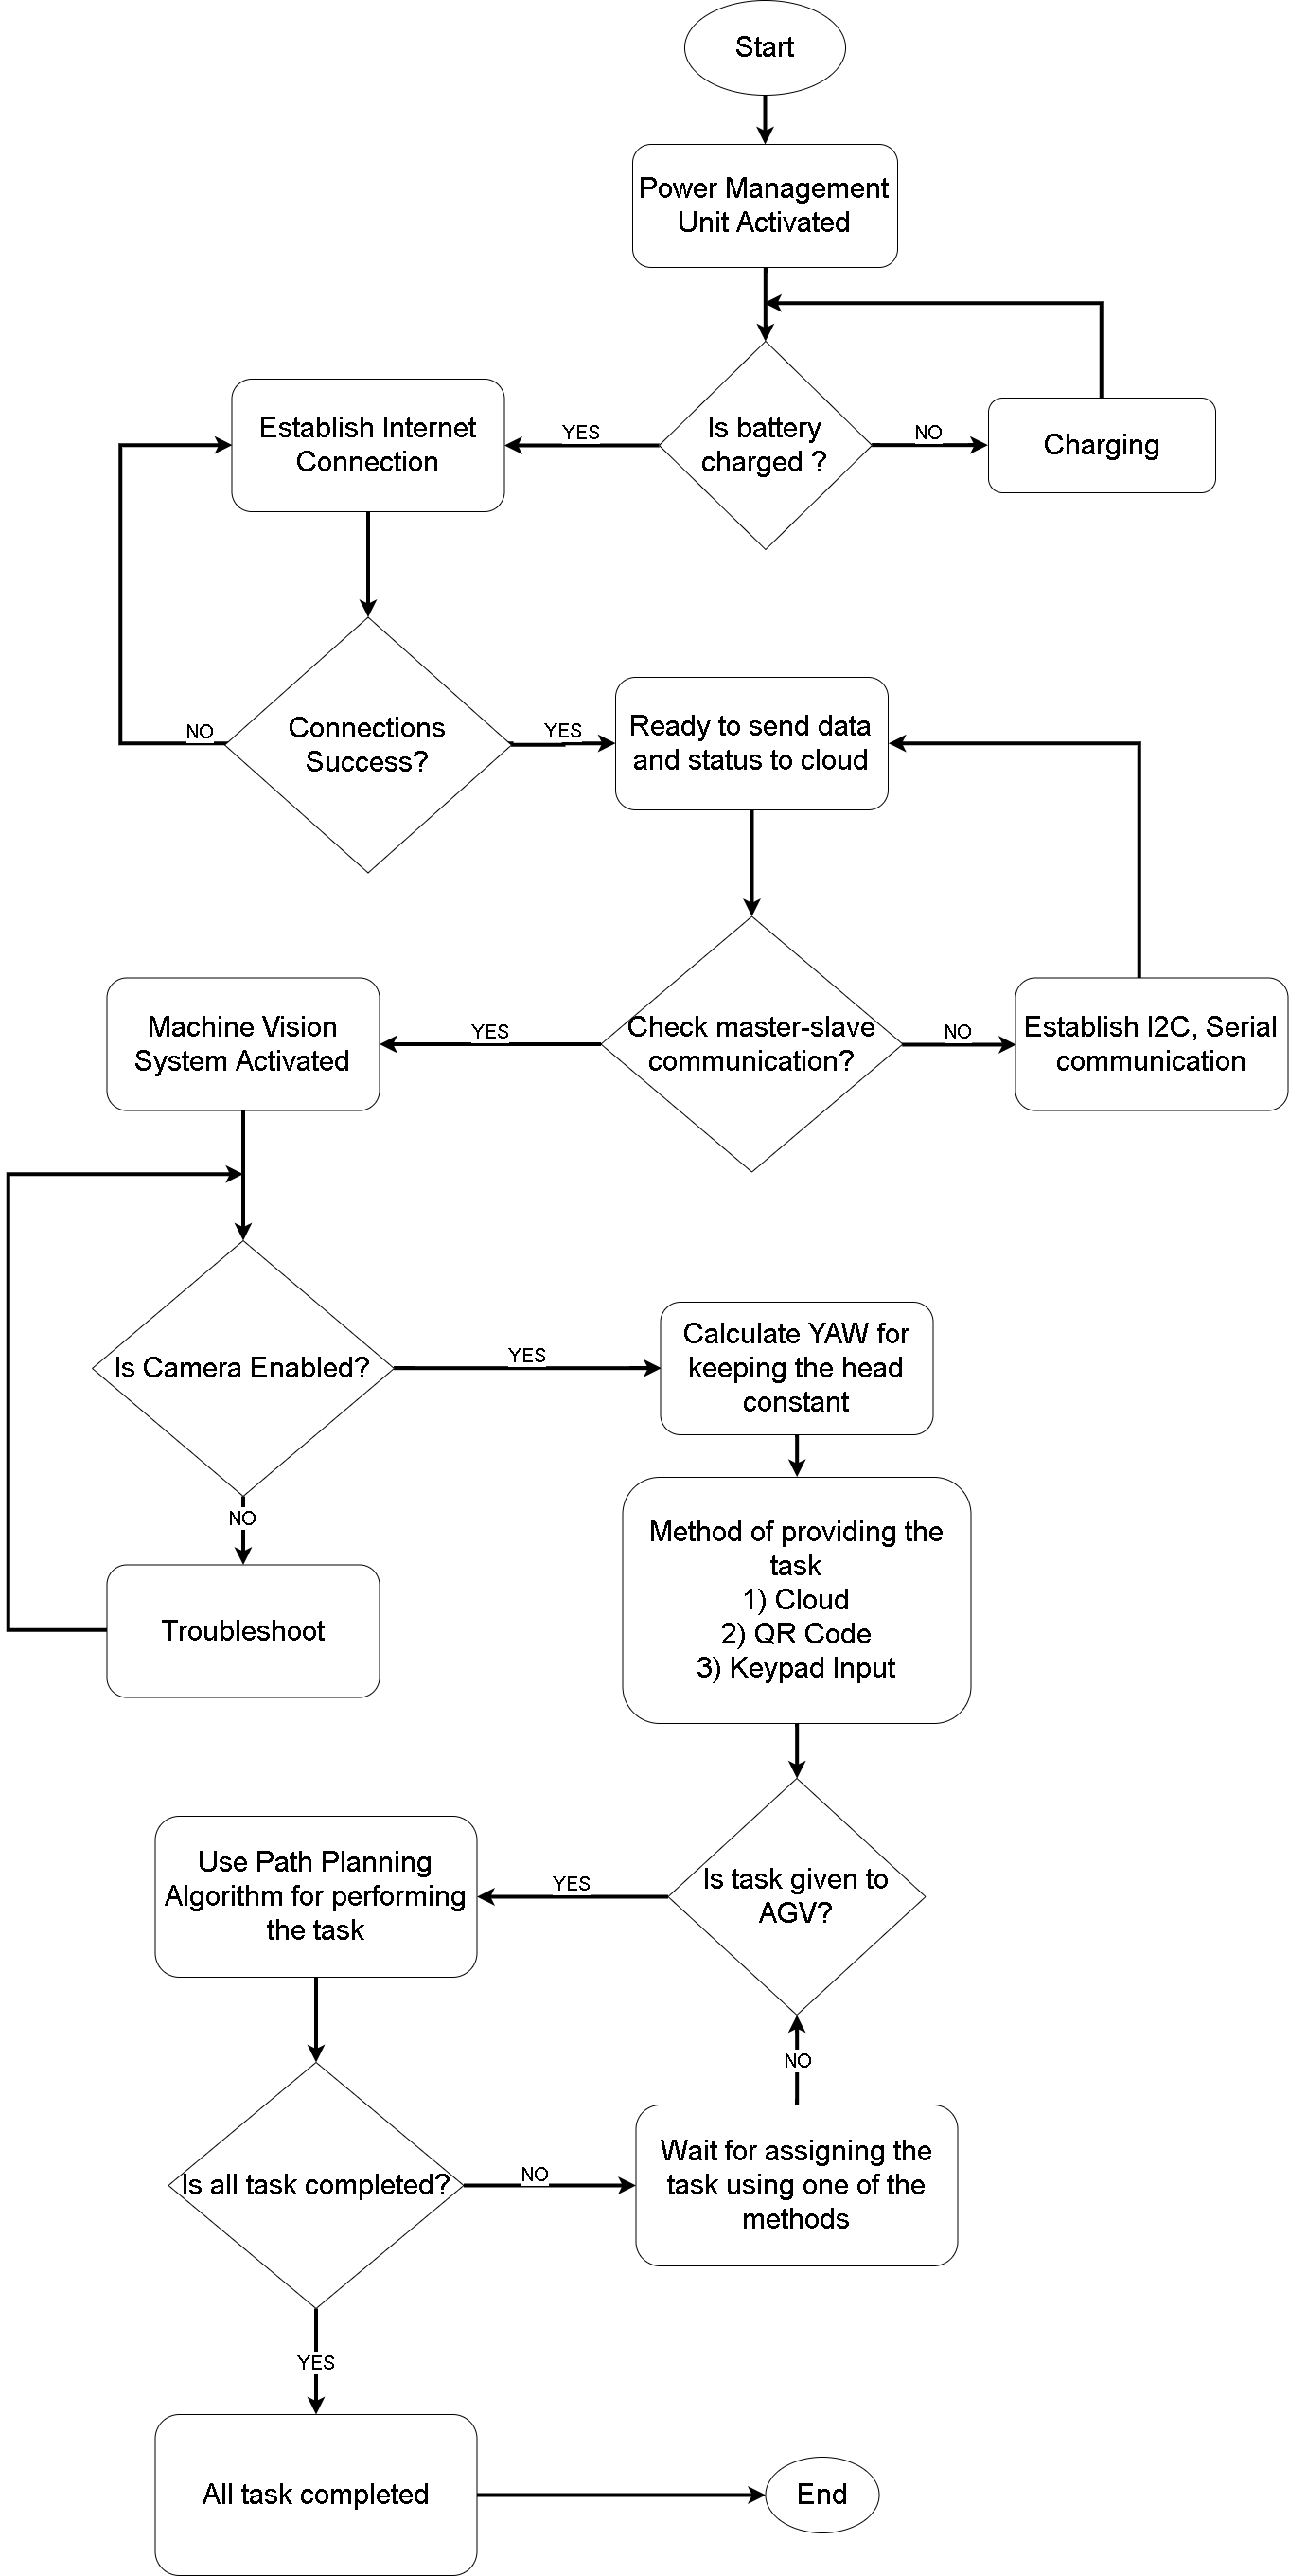
\includegraphics[width =11cm]{project/images/Flowchart.png}
\caption{Flowchart}
\end{figure}
\newpage
\begin{itemize}
    \item  When AGV is turned on, firstly it checks whether the battery is charged or not. If it is not AGV will give alert to the user that the battery level is below the threshold value.
    \item Once the battery is checked, AGV establishes an internet connection in order to manage data, and check whether the connection is successful or not.
    \item When all these primary tasks are completed, AGV is ready to perform the assigned task.
    \item In order to perform a task, it needs to check the controller’s communication with slaves. If it is ok the working continues. And if not it establishes necessary communication.
    \item For the navigation, firstly it enables the webcam and necessary hardware successfully. 
    \item The task can be given to AGV through remote accessing using the cloud, QR code or keypad input.
    \item After that, AGV checks whether the assigned task is completed or not if not completed, it waits till the completion of the task and checks for the next task.
\end{itemize}

%\paragraph{} 

\newpage